\hypertarget{labor-investment}{%
\subsubsection{Labor Investment}\label{labor-investment}}

Question: What was the cost of an organization for its employees to
create the counted contributions (e.g., commits, issues, and pull
requests)?

\hypertarget{description}{%
\paragraph{Description}\label{description}}

Open source projects are often supported by organizations through labor
investment. This metric tracks the monetary investment of organizations
(as evident in labor costs) to individual projects.

\hypertarget{objectives}{%
\paragraph{Objectives}\label{objectives}}

As organizational engagement with open source projects becomes
increasingly important, it is important for organization to clearly
understand their labor investment. The objective of this metric is to
improve transparency in labor costs for organizations engaged with open
source projects. This metric gives an Open Source Program Office (OSPO)
manager a way to compare contributed labor costs across a portfolio of
projects. For example, the Labor Investment metric can be used to
prioritize investment or determine return on investment such as:

\begin{itemize}
\tightlist
\item
  Labor Investment as a means of evaluating OSPO priorities and
  justifying budgets
\item
  Labor Investment as a way to explain product/program management
  priority
\item
  Labor Investment as an argument for the value of continued investing
  in OSPOs
\item
  Labor Investment to report and compare labor costs of contributed vs
  in-house work
\item
  Labor Investment to compare project effectiveness across a portfolio
  of projects
\end{itemize}

\hypertarget{implementation}{%
\paragraph{Implementation}\label{implementation}}

Base metrics include:

\begin{itemize}
\tightlist
\item
  Number of contributions
\item
  Number of contributions broken out by contributor types (internal /
  external)
\item
  Number of contributions broken out by contribution types (e.g.,
  commits, issues, pull requests)
\end{itemize}

Parameters include:

\begin{itemize}
\tightlist
\item
  Hourly labor rate
\item
  Average labor hours to create contribution (by contribution type)
\end{itemize}

Labor Investment = For each contribution type, sum (Number of
contributions * Average labor hours to create contribution * Average
hourly rate)

\hypertarget{filters}{%
\subparagraph{Filters}\label{filters}}

\begin{itemize}
\tightlist
\item
  Internal vs external contributors
\item
  Issue tags
\item
  Project sources (e.g., internal, open-source repos, competitor
  open-source repos)
\end{itemize}

\hypertarget{visualizations}{%
\subparagraph{Visualizations}\label{visualizations}}

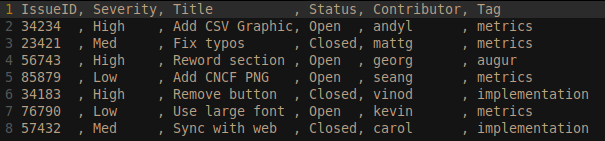
\includegraphics{images/labor-investment_csv.png}

Our first visualization of parameterized metrics rely on CSV exports
that can be made available from Augur. Spreadsheets are used for metric
parameters and calculation formulas. Future implementations may add
features for parameter manipulation directly in the webapp.

\hypertarget{references}{%
\paragraph{References}\label{references}}

\begin{itemize}
\tightlist
\item
  \href{https://www.slideshare.net/caniszczyk/starting-an-open-source-program-office-ospo}{Starting
  an Open Source Program Office}
\item
  \href{https://events19.linuxfoundation.org/wp-content/uploads/2018/07/OSLS_2019-untold-story-of-OSPO.pdf}{Creating
  an Open Source Program Office}
\item
  \href{https://d1.awsstatic.com/Open\%20Source/enterprise-oss-book.pdf}{Open
  Source in the Enterprise}
\end{itemize}
